\documentclass[letter]{article}
\usepackage{natbib}
\usepackage{color}
\definecolor{myurlblue}{rgb}{0.3,0.2,0.7}
\usepackage[colorlinks=true,urlcolor=myurlblue,pagecolor=black,citecolor=myurlblue,linkcolor=black]{hyperref}


\title{Basic Trajectory Analysis with Bio3D}
\author{Barry Grant\\
University of California, San Diego}



\usepackage{Sweave}
\begin{document}
\maketitle
\tableofcontents

\section{Introduction}
The aim of this document, termed a vignette\footnote{This vignette contains executable examples, see \texttt{help(vignette)} for further details.} in R parlance, is to provide a brief task-oriented introduction to basic trajectory analysis with the bio3d R package \citep{grant06}.  A number of other bio3d package vignettes are available, including: \texttt{Bio3D installation and overview}, \texttt{Comparative protein structure analysis with Bio3D} and \texttt{Introduction to sequence conservation analysis with Bio3D}.  In this vignette, \texttt{Basic trajectory analysis with Bio3D}, we will demonstrate the use of several common bio3d facilitates for the analysis of molecular dynamics trajectories.



\paragraph{Supporting Material:}
The latest version, full documentation and furhter vignettes can be obtained from the bio3d website: \href{http://mccammon.ucsd.edu/~bgrant/bio3d/}{http://mccammon.ucsd.edu/$\sim$bgrant/bio3d/} and wiki: \href{http://bio3d.pbwiki.com/}{http://bio3d.pbwiki.com/}.




\subsection{Getting Started}
Start R, load the bio3d package and use the command \texttt{lbio3d()} to list the current functions available within the package:

\begin{Schunk}
\begin{Sinput}
> library(bio3d)
> lbio3d()
\end{Sinput}
\begin{Soutput}
 [1] "aa123"             "aa2index"          "aa321"            
 [4] "aln2html"          "angle.xyz"         "atom.select"      
 [7] "atom2xyz"          "blast.pdb"         "bounds"           
[10] "bwr.colors"        "chain.pdb"         "cmap"             
[13] "consensus"         "conserv"           "convert.pdb"      
[16] "core.find"         "dccm"              "diag.ind"         
[19] "dist.xyz"          "dm"                "dm.xyz"           
[22] "dssp"              "entropy"           "fit.xyz"          
[25] "gap.inspect"       "get.pdb"           "get.seq"          
[28] "ide.filter"        "identity"          "is.gap"           
[31] "lbio3d"            "mktrj.pca"         "mono.colors"      
[34] "motif.find"        "orient.pdb"        "pairwise"         
[37] "pca.project"       "pca.tor"           "pca.xyz"          
[40] "pca.xyz2z"         "pca.z2xyz"         "pdb.summary"      
[43] "pdbaln"            "plot.bio3d"        "plot.blast"       
[46] "plot.core"         "plot.dccm"         "plot.dmat"        
[49] "plot.pca"          "plot.pca.loadings" "plot.pca.score"   
[52] "plot.pca.scree"    "print.core"        "print.pdb"        
[55] "print.rle2"        "read.all"          "read.crd"         
[58] "read.dcd"          "read.fasta"        "read.fasta.pdb"   
[61] "read.ncdf"         "read.pdb"          "read.pdcBD"       
[64] "read.pqr"          "rle2"              "rmsd"             
[67] "rmsd.filter"       "rmsf"              "rot.lsq"          
[70] "seq.pdb"           "seq2aln"           "seqaln"           
[73] "seqaln.pair"       "seqbind"           "split.pdb"        
[76] "store.atom"        "stride"            "torsion.pdb"      
[79] "torsion.xyz"       "trim.pdb"          "unbound"          
[82] "vec2resno"         "wiki.tbl"          "wrap.tor"         
[85] "write.crd"         "write.fasta"       "write.ncdf"       
[88] "write.pdb"         "write.pqr"        
\end{Soutput}
\end{Schunk}
Detailed documentation and example code for each function can be accessed via the \texttt{help()} and \texttt{example()} commands (e.g. \texttt{help(read.pdb)}).  You can also copy and paste any of the example code from the documentation of a particular function, or indeed this vignette, directly into your R session.

\section{Reading Example Trajectory Data}
A number of example data sets are shipped with the bio3d package. The main purpose of including this data is to allow users to more quickly appreciate the capabilities of various bio3d functions that would otherwise require potentially time consuming data generation. In the examples below we will input, process and analyze a molecular dynamics trajectory of human immunodeficiency virus aspartic protease (HIV PR). This trajectory is stored in CHARMM/NAMD dcd format and has had all solvent and non C-alpha protein atoms excluded to reduce overall file size.


The code snippet below sets the file paths for the example HIV PR starting structure (pdbfile) and trajectory data (dcdfile).
\begin{Schunk}
\begin{Sinput}
> dcdfile <- system.file("examples/hivp.dcd", package = "bio3d")
> pdbfile <- system.file("examples/hivp.pdb", package = "bio3d")
\end{Sinput}
\end{Schunk}
Note that in the above example the \texttt{system.file()} command returns a character string corresponding to the file name of a PDB structure included with the bio3d package. This is required as users may install the package in different locations. When using your own input files the \texttt{system.file()} command will not be required, for example

\begin{Schunk}
\begin{Sinput}
> mydcdfile <- "/path/to/my/data/myfile.dcd"
\end{Sinput}
\end{Schunk}

\begin{Schunk}
\begin{Sinput}
> dcd <- read.dcd(dcdfile)
\end{Sinput}
\begin{Soutput}
 NATOM = 198 
 NFRAME= 351 
 ISTART= 0 
 last  = 351 
 nstep = 351 
 nfile = 351 
 NSAVE = 1 
 NDEGF = 0 
 version 24 
Reading (x100)...done
\end{Soutput}
\begin{Sinput}
> pdb <- read.pdb(pdbfile)
\end{Sinput}
\end{Schunk}
The \texttt{read.dcd()} and \texttt{read.pdb()} commands processes the input files and returns their output to the objects \texttt{dcd} and \texttt{pdb}. We can check the basic structure of these objects with the following commands:

\begin{Schunk}
\begin{Sinput}
> pdb.summary(pdb)
\end{Sinput}
\begin{Soutput}
..| segid |..
total #: 1 
values : NA 


..| chain |..
total #: 2 
values : A B 


..| resno |..
total #: 198 
in segments: 

  start end length
1     1  99     99
2     1  99     99


..| resid |..
total #: 20 ( diff types from 198 )
values : 

ALA ARG ASN ASP CYS GLN GLU GLY HIS ILE LEU LYS MET PHE PRO SER THR TRP TYR VAL 
  6   8   6   8   4  12   8  26   2  26  24  12   4   4  12   2  16   4   2  12 


..| eleno |..
total # : 198 
in segments: 

  start end length
1     1 198    198


..| elety |..
total # : 1 ( diff types from 198 )
values : 

 CA 
198 


..| summary |..
atom     #: 198 
xyz      #: 594 
calpha   #: 198 
sequence #: PQITLWQRPLVTIKIGGQLKEALLDTGADDTVLEEMSLPGRWKPKMIGGIGGFIKVRQYDQILIEICGHKAIGTVLVGPTPVNIIGRNLLTQIGCTLNFPQITLWQRPLVTIKIGGQLKEALLDTGADDTVLEEMSLPGRWKPKMIGGIGGFIKVRQYDQILIEICGHKAIGTVLVGPTPVNIIGRNLLTQIGCTLNF 
\end{Soutput}
\begin{Sinput}
> length(pdb$xyz)
\end{Sinput}
\begin{Soutput}
[1] 594
\end{Soutput}
\begin{Sinput}
> dim(dcd)
\end{Sinput}
\begin{Soutput}
[1] 351 594
\end{Soutput}
\end{Schunk}
Note that the output of the \texttt{dim()} function is telling us that we have 351 trajectroy frames (or rows in our dcd matrix) and 594 coordinates (or x, y and z columns).

\section{Trajectory Frame Superposition}
In this simple example we select all C-alpha atoms for trajectory frame superposition.
\begin{Schunk}
\begin{Sinput}
> ca.inds <- atom.select(pdb, elety = "CA")
\end{Sinput}
\begin{Soutput}
      segid chain resno resid eleno elety
Stest ""    ""    ""    ""    ""    "CA" 
Natom "198" "198" "198" "198" "198" "198"
 *  Selected a total of: 198 intersecting atoms  *
\end{Soutput}
\end{Schunk}
The returned \texttt{ca.inds} object is a list containing atom and xyz numeric indices that we can now use to superpose all frames of the trajectory on the selected indices (in this case corresponding to all alpha Carbon atoms) with the \texttt{fit.xyz()} function.
\begin{Schunk}
\begin{Sinput}
> xyz <- fit.xyz(fixed = pdb$xyz, mobile = dcd, fixed.inds = ca.inds$xyz, 
+     mobile.inds = ca.inds$xyz)
\end{Sinput}
\end{Schunk}
The above command performs the actual superposition and stores the new coordinates in the matrix object \texttt{xyz}.

\section{Root Mean Square Deviation (RMSD)}
RMSD is a standard measure of structural distance between coordinate sets and is implemented in the bio3d function \texttt{rmsd()}.

\begin{Schunk}
\begin{Sinput}
> rd <- rmsd(xyz[1, ca.inds$xyz], xyz[, ca.inds$xyz])
> plot(rd, typ = "l", ylab = "RMSD", xlab = "Frame No.")
> points(lowess(rd), typ = "l", col = "red", lty = 2, lwd = 2)
\end{Sinput}
\end{Schunk}
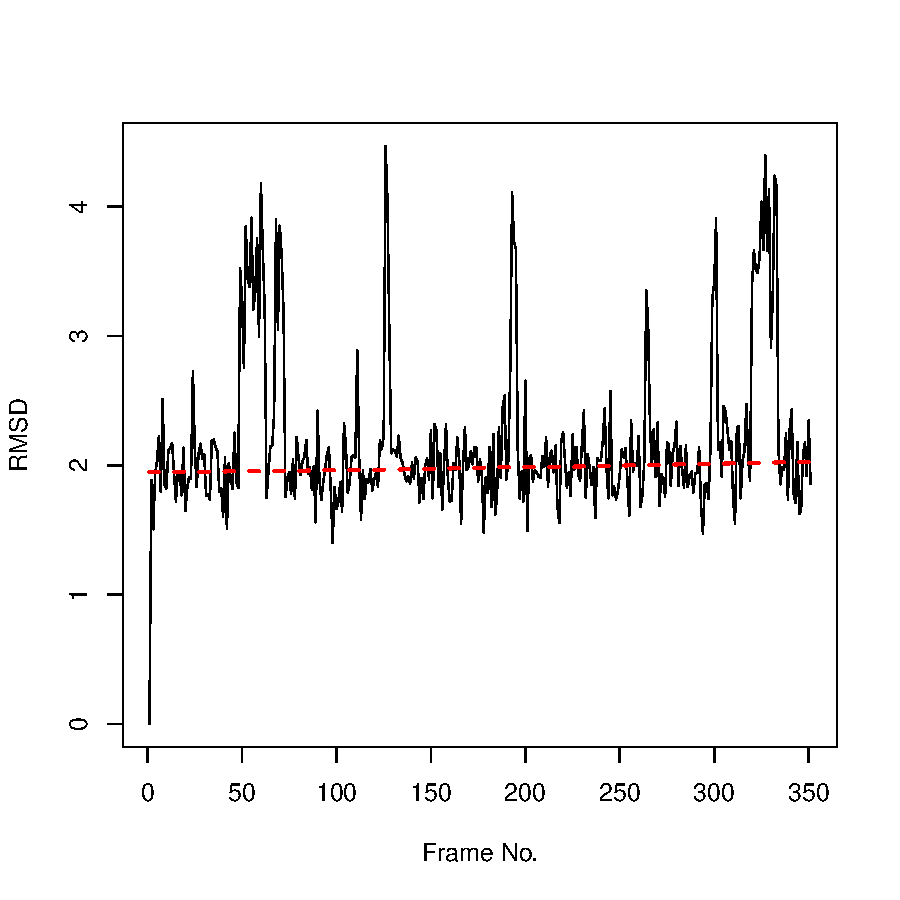
\includegraphics{Bio3D_trajectory-008}

A quick histogram can be useful for examining the distribution of RMSD values.
\begin{Schunk}
\begin{Sinput}
> hist(rd, breaks = 40, freq = FALSE, main = "RMSD Histogram")
> lines(density(rd), col = "gray", lwd = 3)
\end{Sinput}
\end{Schunk}
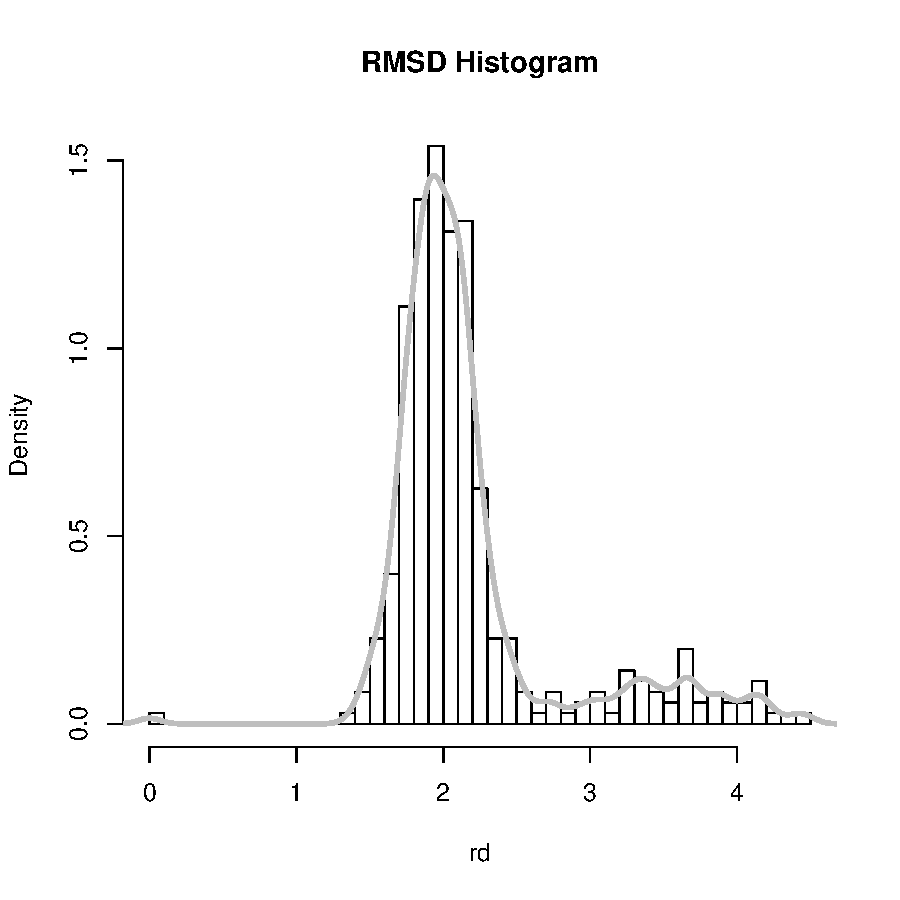
\includegraphics{Bio3D_trajectory-009}

\begin{Schunk}
\begin{Sinput}
> summary(rd)
\end{Sinput}
\begin{Soutput}
   Min. 1st Qu.  Median    Mean 3rd Qu.    Max. 
  0.000   1.852   2.020   2.183   2.216   4.468 
\end{Soutput}
\end{Schunk}

\section{Root Mean Squared Fluctuations (RMSF)}
RMSF is an often used measure of conformational variance and is implemented in the bio3d function \texttt{rmsf()}.
\begin{Schunk}
\begin{Sinput}
> rf <- rmsf(xyz[, ca.inds$xyz])
> plot(rf, ylab = "RMSF", xlab = "Residue Position", typ = "l")
\end{Sinput}
\end{Schunk}
\includegraphics{Bio3D_trajectory-011}

\section{Principal Component Analysis}
PCA can be employed to examine the relationship between different conformations sampled during the trajectory and is implemented in the bio3d functions \texttt{pca.xyz()} and \texttt{pca.tor()}. The application of PCA to both distributions of experimental structures and molecular dynamics trajectories, along with its ability to provide considerable insight into the nature of conformational differences has been discussed previously (see \citet{grant06} and references therein). 

Briefly, the resulting principal components (orthogonal eigenvectors) describe the axes of maximal variance of the distribution of structures. Projection of the distribution onto the subspace defined by the largest principal components results in a lower dimensional representation of the structural dataset. The percentage of the total mean square displacement (or variance) of atom positional fluctuations captured in each dimension is characterized by their corresponding eigenvalue (see the next figure). Experience suggests that 3--5 dimensions are often sufficient to capture over 70 percent of the total variance in a given family of experimental structures or indeed a standard molecular dynamics trajectory. Thus, a handful of principal components are sufficient to provide a useful description while still retaining most of the variance in the original distribution \citet{grant06}.

A quick overview of the results of \texttt{pca.xyz()} can be obtained by calling \texttt{plot.pca()}
\begin{Schunk}
\begin{Sinput}
> pc <- pca.xyz(xyz[, ca.inds$xyz])
> plot(pc, col = bwr.colors(nrow(xyz)))
\end{Sinput}
\end{Schunk}
\includegraphics{Bio3D_trajectory-012}

Note that there are distinct groupings of conformations along the PC1 plane (one centered around -30 and a second, larger grouping, at +5). The continuous color scale (from blue to whit to red) indicates that there are periodic jumps between these conformers throughout the trajectory. Below we perform a quick clustering in PC-space to further highlight these distinct conformers.
\begin{Schunk}
\begin{Sinput}
> hc <- hclust(dist(pc$z[, 1:2]))
> grps <- cutree(hc, k = 2)
> plot(pc, col = grps)
\end{Sinput}
\end{Schunk}
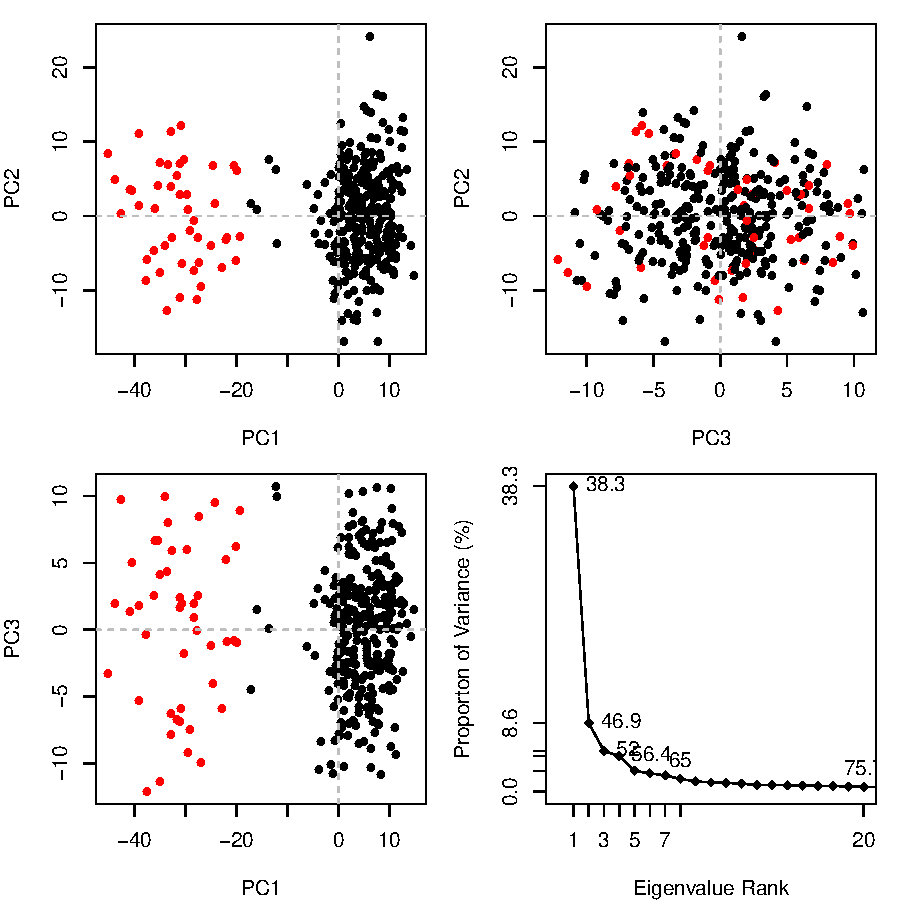
\includegraphics{Bio3D_trajectory-013}

Bellow we call \texttt{plot.bio3d()} to examine the contribution of each residue to the first two principal components.

\begin{Schunk}
\begin{Sinput}
> plot.bio3d(pc$au[, 1], ylab = "PC1 (A)", xlab = "Residue Position", 
+     typ = "l")
> points(pc$au[, 2], typ = "l", col = "blue")
\end{Sinput}
\end{Schunk}
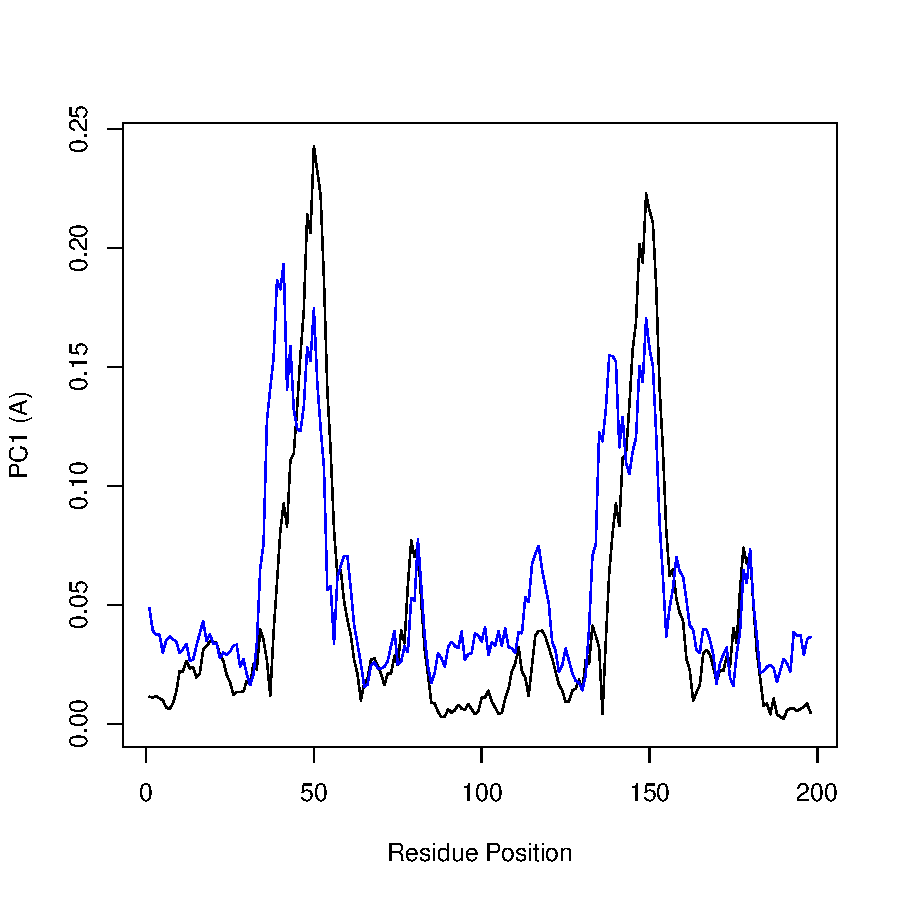
\includegraphics{Bio3D_trajectory-014}

To further aid interpretation, a PDB format trajectory can be produced that interpolates between the most dissimilar structures in the distribution along a given principal component.  This involves dividing the difference between the conformers into a number of evenly spaced steps along the principal components, forming the frames of the output multi-model PDB trajectory. Such trajectories can be directly visualized in a molecular graphics program, such as VMD \citep{vmd}. Furthermore, the interpolated structures can be analyzed for possible domain and shear movements with other bio3d functions, or used as initial seed structures for more advanced reaction path refinement methods (note you will likely want to perform all heavy atom PCA for such applications).
\begin{Schunk}
\begin{Sinput}
> p1 <- mktrj.pca(pc, pc = 1, b = pc$au[, 1], file = "pc1.pdb")
> p2 <- mktrj.pca(pc, pc = 2, b = pc$au[, 2], file = "pc2.pdb")
\end{Sinput}
\end{Schunk}

You can also write these trajectory's as AMBER NetCDF format files with the \texttt{write.ncdf} function.
\begin{Schunk}
\begin{Sinput}
> write.ncdf(p1, "trj_pc1.nc")
\end{Sinput}
\end{Schunk}
\begin{center}
\includegraphics[width=120mm]{hiv_pc1.png}
\end{center}


\section{Cross-Correlation Analysis}
The extent to which the atomic fluctuations/displacements of a system are correlated with one another can be assessed by examining the magnitude of all pairwise cross-correlation coefficients. The Bio3D \texttt{dccm()} function returns a matrix of all atom-wise cross-correlations whose elements may be displayed in a graphical representation frequently termed a dynamical cross-correlation map, or DCCM.

\begin{Schunk}
\begin{Sinput}
> cij <- dccm(xyz[, ca.inds$xyz])
> plot.dccm(cij)
\end{Sinput}
\end{Schunk}
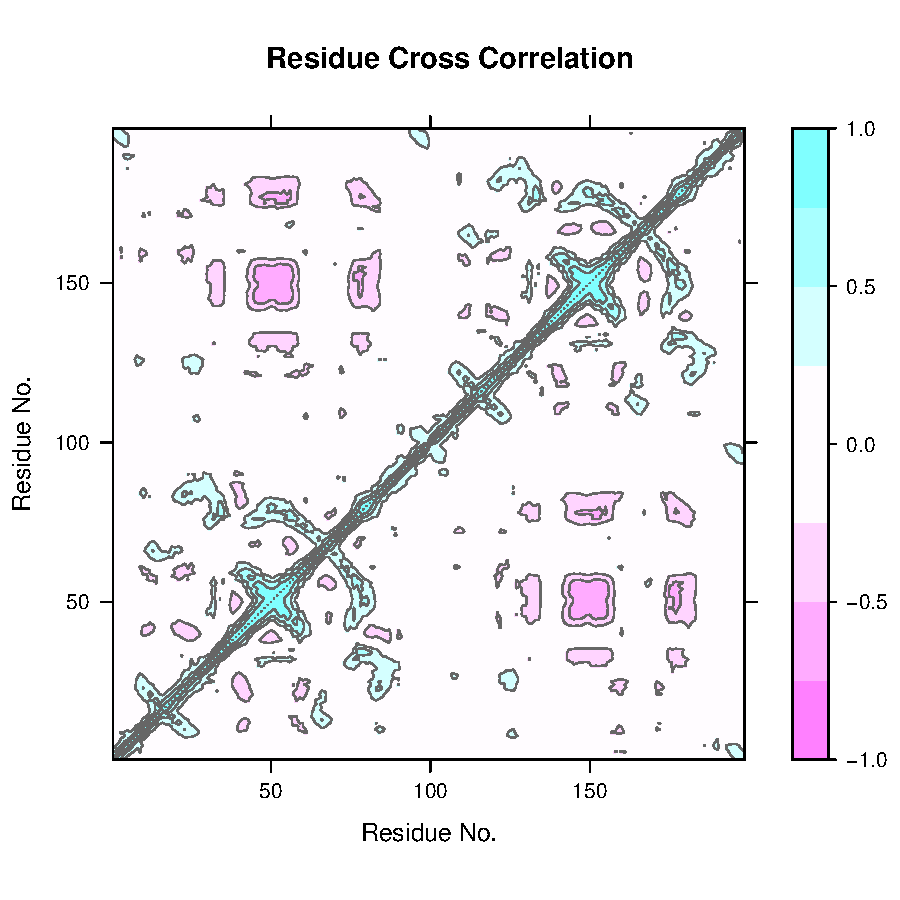
\includegraphics{Bio3D_trajectory-017}

\section*{Session Info}
\begin{Schunk}
\begin{Sinput}
> toLatex(sessionInfo())
\end{Sinput}
\begin{Soutput}
\begin{itemize}\raggedright
  \item R version 2.13.0 (2011-04-13), \verb|x86_64-unknown-linux-gnu|
  \item Locale: \verb|LC_CTYPE=en_US.UTF-8|, \verb|LC_NUMERIC=C|, \verb|LC_TIME=en_US.UTF-8|, \verb|LC_COLLATE=en_US.UTF-8|, \verb|LC_MONETARY=C|, \verb|LC_MESSAGES=en_US.UTF-8|, \verb|LC_PAPER=en_US.UTF-8|, \verb|LC_NAME=C|, \verb|LC_ADDRESS=C|, \verb|LC_TELEPHONE=C|, \verb|LC_MEASUREMENT=en_US.UTF-8|, \verb|LC_IDENTIFICATION=C|
  \item Base packages: base, datasets, graphics, grDevices, grid,
    methods, stats, utils
  \item Other packages: bio3d~1.1-4, lattice~0.19-23
  \item Loaded via a namespace (and not attached): tools~2.13.0
\end{itemize}
\end{Soutput}
\end{Schunk}

\begin{thebibliography}{9}


\bibitem[Grant \emph{et al.}, 2006]{grant06}
Grant, B.J. and Rodrigues, A.P.D.C and Elsawy, K.M. and Mccammon, A.J. and Caves, L.S.D. (2006)
\textbf{Bio3d: an R package for the comparative analysis of protein structures.}
\emph{Bioinformatics},
\textbf{22}, 2695--2696.


\bibitem[Humphrey \emph{et al.}, 1996]{vmd}
Humphrey, W., et al. (1996)
\textbf{VMD: visual molecular dynamics.}
\emph{J. Mol. Graph}, \textbf{14}, 33--38


\end{thebibliography}

\end{document}

